\PassOptionsToPackage{unicode=true}{hyperref} % options for packages loaded elsewhere
\PassOptionsToPackage{hyphens}{url}
\PassOptionsToPackage{dvipsnames,svgnames*,x11names*}{xcolor}
%
\documentclass[]{report}
\usepackage{lmodern}
\usepackage{amssymb,amsmath}
\usepackage{ifxetex,ifluatex}
\usepackage{fixltx2e} % provides \textsubscript
\ifnum 0\ifxetex 1\fi\ifluatex 1\fi=0 % if pdftex
  \usepackage[T1]{fontenc}
  \usepackage[utf8]{inputenc}
  \usepackage{textcomp} % provides euro and other symbols
\else % if luatex or xelatex
  \usepackage{unicode-math}
  \defaultfontfeatures{Ligatures=TeX,Scale=MatchLowercase}
\fi
% use upquote if available, for straight quotes in verbatim environments
\IfFileExists{upquote.sty}{\usepackage{upquote}}{}
% use microtype if available
\IfFileExists{microtype.sty}{%
\usepackage[]{microtype}
\UseMicrotypeSet[protrusion]{basicmath} % disable protrusion for tt fonts
}{}
\IfFileExists{parskip.sty}{%
\usepackage{parskip}
}{% else
\setlength{\parindent}{0pt}
\setlength{\parskip}{6pt plus 2pt minus 1pt}
}
\usepackage{xcolor}
\usepackage{hyperref}
\hypersetup{
            pdftitle={Transfer of Status Report},
            pdfauthor={Nilo M. Recalde},
            colorlinks=true,
            linkcolor=Maroon,
            filecolor=Maroon,
            citecolor=Blue,
            urlcolor=Blue,
            breaklinks=true}
\urlstyle{same}  % don't use monospace font for urls
\usepackage{longtable,booktabs}
% Fix footnotes in tables (requires footnote package)
\IfFileExists{footnote.sty}{\usepackage{footnote}\makesavenoteenv{longtable}}{}
\usepackage{graphicx,grffile}
\makeatletter
\def\maxwidth{\ifdim\Gin@nat@width>\linewidth\linewidth\else\Gin@nat@width\fi}
\def\maxheight{\ifdim\Gin@nat@height>\textheight\textheight\else\Gin@nat@height\fi}
\makeatother
% Scale images if necessary, so that they will not overflow the page
% margins by default, and it is still possible to overwrite the defaults
% using explicit options in \includegraphics[width, height, ...]{}
\setkeys{Gin}{width=\maxwidth,height=\maxheight,keepaspectratio}
\setlength{\emergencystretch}{3em}  % prevent overfull lines
\providecommand{\tightlist}{%
  \setlength{\itemsep}{0pt}\setlength{\parskip}{0pt}}
\setcounter{secnumdepth}{0}
% Redefines (sub)paragraphs to behave more like sections
\ifx\paragraph\undefined\else
\let\oldparagraph\paragraph
\renewcommand{\paragraph}[1]{\oldparagraph{#1}\mbox{}}
\fi
\ifx\subparagraph\undefined\else
\let\oldsubparagraph\subparagraph
\renewcommand{\subparagraph}[1]{\oldsubparagraph{#1}\mbox{}}
\fi

% set default figure placement to htbp
\makeatletter
\def\fps@figure{htbp}
\makeatother

\usepackage{fontspec}
\setmainfont[Ligatures=TeX,Scale=1]{Lato}
\usepackage{leading}
\leading{18pt}
\usepackage{sectsty}
\chapterfont{\raggedleft}

\title{Transfer of Status Report}
\author{Nilo M. Recalde}
\date{Last compiled on 18 October, 2020}

\begin{document}
\maketitle

{
\hypersetup{linkcolor=}
\setcounter{tocdepth}{2}
\tableofcontents
}
\listoffigures
\hypertarget{introduction}{%
\chapter{Introduction}\label{introduction}}

\hypertarget{general-introduction}{%
\section{General introduction}\label{general-introduction}}

\begin{quote}
\emph{Definitely not a placeholder for a Darwin quote}
\end{quote}

\hypertarget{animal-culture-and-social-learning}{%
\subsection{Animal culture and social
learning}\label{animal-culture-and-social-learning}}

Culture was once considered the sole domain of humans. Over the past few
decades this view has been steadily challenged, and today it is common
to find allusions to non-human animal cultures in scientific journals
and the popular press alike. To be sure, some energetically oppose the
notion, and there is no shortage of disagreement over the very
definition of the term `culture'. But an increasing number of students
of behaviour and evolution suspect that, intricate and distinctive as
human culture might be, the difference must be one of degree---not kind.

What constitutes culture, then? For our purposes, we can define it as
any behavioural trait that is maintained in a population by virtue of
being learnt from others; not genetically inherited, nor individually
acquired. (see definitions in Whiten et al.
\protect\hyperlink{ref-Whiten2017}{2017}; Laland \& Hoppitt
\protect\hyperlink{ref-Laland2003}{2003}.) Human ritual funerary
practices are cultural, so is the game of croquet. And, under this
definition, so are tool use in capuchin monkeys, homing efficiency in
pigeons, the songs of many birds, some feeding behaviours in humpback
whales, and even mate preferences in fruit flies ({\textbf{???}}; Slater
\protect\hyperlink{ref-Slater2003}{2003}; Allen et al.
\protect\hyperlink{ref-Allen2013a}{2013}; Sasaki \& Biro
\protect\hyperlink{ref-Sasaki2017a}{2017}; Falótico et al.
\protect\hyperlink{ref-Falotico2019}{2019}).

Social learning is ubiquitous among animals, and a prerequisite for
culture. Although it may not always be beneficial (Henrich \& Boyd
\protect\hyperlink{ref-Henrich1998}{1998}; Giraldeau et al.
\protect\hyperlink{ref-Giraldeau2002}{2002}; Whitehead \& Richerson
\protect\hyperlink{ref-Whitehead2009}{2009}), there is ample evidence
that many of the things that many animals must learn to survive and
reproduce can only be acquired by observing or interacting with others
(Galef \& Laland \protect\hyperlink{ref-Galef2005}{2005}). Learning will
happen more often from animals that are closer in space or in a social
group, and this inevitable fact creates opportunities for behaviours to
change differently in different populations, sometimes becoming better
suited to local conditions. When these differences---beneficial or
not---accumulate and persist over time, a cultural tradition is born.

Whether found in humans or other animals, cultures can be transient or
long-lasting, disorderly diverse or monolithically uniform. To give two
primate examples, chimpanzees (\emph{Pan troglodytes}) may have used
stone tools in a similar way for thousands of years (Mercader et al.
\protect\hyperlink{ref-Mercader2007}{2007}; Carvalho et al.
\protect\hyperlink{ref-Carvalho2008}{2008}), and white-faced capuchin
monkeys (\emph{Cebus capucinus}) frequently invent and abandon quirky
social conventions such as eyeball-poking, handsniffing and tail-sucking
(Perry et al. \protect\hyperlink{ref-Perry2003}{2003}).

\hypertarget{cultural-evolution-in-birds}{%
\subsection{Cultural evolution in
birds}\label{cultural-evolution-in-birds}}

(For a recent review see Aplin \protect\hyperlink{ref-Aplin2018}{2019})

This section will bridge the very general introduction above and the
more specific overview of bird song below, as well as justify why birds
are a good system at all.

Socially acquired acoustic signals, such as the song of humpback whales
and oscine songbirds, offer incredibly valuable opportunities for
answering some of these questions. Songs can convey information about
the identity and social position of signallers; they are moulded by
natural and sexual selection, stochastic processes and directional
cultural change, and, crucially, can be recorded and analysed in minute
detail.

And now comes a brief introduction to song:

\hypertarget{bird-song-a-short-introduction}{%
\section{Bird song: a short
introduction}\label{bird-song-a-short-introduction}}

\hypertarget{historical}{%
\subsubsection{Historical}\label{historical}}

Brief introduction to the long history of the study of bird song.
Mention Barrington, Marler, Thorpe, Nottebohm, etc., but focus more on
how research interests have shifted over the past 50 years or so.

\hypertarget{why-sing}{%
\subsubsection{Why sing?}\label{why-sing}}

Overview of some of the ultimate causes that might be responsible the
evolution of singing in birds, and some of the functions that it may
serve in different taxa.

\hypertarget{song-learning-in-phylogenetic-perspective}{%
\subsubsection{Song learning in phylogenetic
perspective}\label{song-learning-in-phylogenetic-perspective}}

Most birds vocalise, but song learning has only evolved in three orders
(Psittaciformes, Apodiformes, and Passeriformes). Within the passerines,
oscines learn their songs, while suboscines do not. Briefly, why might
social acquisition of song evolve?

\hypertarget{song-structure-and-syntax}{%
\subsubsection{Song structure and
syntax}\label{song-structure-and-syntax}}

Among the birds that learn their songs, there is a fantastic range of
variation in repertoire size and complexity. A brief overview of work
done on the diverse syntactic structures of bird songs, small-world
organisation, hierarchical and Markovian organisation, etc.

\hypertarget{some-of-the-forces-that-shape-bird-song}{%
\section{(Some of) The forces that shape bird
song}\label{some-of-the-forces-that-shape-bird-song}}

First I will discuss, in this order, physiological constraints and
phylogenetic inertia, ecological factors, and sexual selection. These
are very important but not the focus of my research. I will then
introduce some ideas about cultural transmission dynamics, innate biases
and spatial, social and demographic factors, which I will explore
throughout the thesis.

\hypertarget{physiological-constraints-and-phylogenetic-inertia}{%
\subsubsection{Physiological constraints and phylogenetic
inertia}\label{physiological-constraints-and-phylogenetic-inertia}}

Bio-mechanics of song production and perceptual/cognitive factors
determine the degrees of freedom available to the rest of processes.

\hypertarget{ecological-factors}{%
\subsubsection{Ecological factors}\label{ecological-factors}}

One of the areas most extensively researched; sensory drive and so on.

\hypertarget{sexual-selection}{%
\subsubsection{Sexual selection}\label{sexual-selection}}

Another aspect to which much attention has been paid: how mate choice
and competition might select for song complexity and repertoire sharing.

\hypertarget{cultural-transmission-dynamics}{%
\subsubsection{Cultural transmission
dynamics}\label{cultural-transmission-dynamics}}

Model biases, song content and structure biases, and changes that occur
as a direct consequence of transmission. General learning strategies,
emphasising the role of conformist learning. Discuss the model of
overproduction and selective attrition.

\hypertarget{the-interplay-of-innate-biases-and-social-learning}{%
\subsubsection{The interplay of innate biases and social
learning}\label{the-interplay-of-innate-biases-and-social-learning}}

A brief discussion contrasting a) the emphasis placed by some authors on
high-fidelity learning with b) ideas more along the lines of Cecilia
Heyes and the french in explaining cultural stability.

Also briefly introduce the experiments of Tchernichovski, Feher et al in
light of ideas about convergent transformation.

And Mets \& Brainard (\protect\hyperlink{ref-Mets2019}{2019}), Mets \&
Brainard (\protect\hyperlink{ref-Mets2017}{2017}) and James et al.
(\protect\hyperlink{ref-James2020}{2020}), etc., on genetically
inherited learning tendencies and the role of experience.

\hypertarget{spatial-social-and-demographic-factors}{%
\subsubsection{Spatial, social and demographic
factors}\label{spatial-social-and-demographic-factors}}

How do habitat geometry, social network topology, population size,
patterns of dispersal, and turnover influence learning opportunities and
contribute to shaping song diversity and evolution?

\hypertarget{polymorphic-song-cultures}{%
\subsubsection{Polymorphic song
cultures}\label{polymorphic-song-cultures}}

Some bird species maintain highly polymorphic song cultures (this is the
case of great tits). Songs are caught between divergent forces (e.g.,
copying errors) and convergence (due to both learning and convergent
transformation, the latter as a consequence of the amplification of
innate perceptual/cognitive biases); their interplay bounds the
diversity available to other processes. Tchernichovski et al.
(\protect\hyperlink{ref-Tchernichovski2017a}{2017}) propose that, at
least some species, `cultural' balancing (negatively
frequency-dependent) selection could play an important role. It also
seems likely that in some or many cases this could simply be a
by-product of the spatial distribution of learners that learn a small
number of song types from different tutors.

\hypertarget{introduction-to-the-study-system}{%
\section{Introduction to the study
system}\label{introduction-to-the-study-system}}

\hypertarget{great-tits}{%
\subsubsection{Great tits}\label{great-tits}}

Biology of the species and some of the work done with great tit song,
especially here in Wytham (e.g., Hunter \& Krebs
\protect\hyperlink{ref-Hunter1979}{1979}; Krebs et al.
\protect\hyperlink{ref-Krebs1978}{1978}; McGregor \& Krebs
\protect\hyperlink{ref-McGregor1982}{1982},
\protect\hyperlink{ref-McGregor1989}{1989}; Fayet et al.
\protect\hyperlink{ref-Fayet2014}{2014}).

\hypertarget{concrete-aims}{%
\section{Concrete aims}\label{concrete-aims}}

This report aims to do the following:

\begin{itemize}
\item
  Provide a broad overview of the framework and the kinds of questions
  that my thesis will try to answer
  (\protect\hyperlink{introduction}{Introduction}).
\item
  Detail some of the methods that I am using to study large amounts of
  song data in an unsupervised way
  (\protect\hyperlink{Methods}{Methods}).
\item
  Summarise the dataset acquired during the 2020 breeding season
  (\protect\hyperlink{Results-and-discussion}{Results}).
\item
  Present an updated plan for next year's field season
  (\protect\hyperlink{Data-collection-plan-for-2021}{2021 plan}).
\item
  Introduce a possible outline for the thesis
  (\protect\hyperlink{Thesis-plan}{Thesis plan}).
\end{itemize}

\hypertarget{methods}{%
\chapter{Methods}\label{methods}}

\hypertarget{study-system}{%
\section{Study system}\label{study-system}}

The study was carried out in Wytham Woods, Oxfordshire, UK (51°46′N,
1°20′W). Wytham woods is a semi-natural deciduous woodland, around 415
hectares in extension, which is surrounded by farmland. Here, a
population of great tits is monitored as part of a long-term survey that
began in 1947. The majority of great tits nests in nestboxes with known
locations. Every year, fieldworkers record the identities of breeding
males and females, the dates of clutch initiation and egg hatching,
clutch size, and fledgling success under standardised protocols. A large
proportion of birds in the population are fitted with a unique British
Trust for Ornithology (BTO) metal leg ring either as nestlings or as
adults. During the breeding season, from March to June, great tit pairs
are socially monogamous and defend territories around their nestboxes
(Hinde \protect\hyperlink{ref-Hinde1952}{1952}).

\hypertarget{song-recording}{%
\section{Song recording}\label{song-recording}}

Every nestbox in the study site is checked by fieldworkers at least once
a week before and during egg laying, which can last from one to 14 days
(Perrins \protect\hyperlink{ref-Perrins1965}{1965}). When a nestbox was
marked as having great tit activity, which usually coincided with the
laying of the first eggs, I placed an autonomous sound recorder in the
vicinity of the nestbox---either in the same tree or in a suitable
neighbouring tree. I recorded birds in this manner from early April
until mid-May, leaving each recorder in the same location for three
consecutive days before moving it to a different nestbox. I relocated
ten recorders every day throughout the duration of the recording period.

I used 30 AudioMoth recorders (Hill et al.
\protect\hyperlink{ref-Hill2019b}{2019}), which were housed in
waterproof, custom-built enclosures (See Fig X). Recording began
approximately one hour before sunrise (\textasciitilde{} 05:36 -- 04:00
UTC) and consisted of seven 59-minute-long recordings with a sample rate
of 48 kHz.

\hypertarget{definitions}{%
\section{Definitions}\label{definitions}}

There is not a consistent set of terms used to refer to the different
levels at which the acoustic output of a bird can be described. For
clarity, these are the definitions that I use throughout this work:

\begin{longtable}[]{@{}ll@{}}
\toprule
\begin{minipage}[b]{0.17\columnwidth}\raggedright
Term\strut
\end{minipage} & \begin{minipage}[b]{0.77\columnwidth}\raggedright
Definition\strut
\end{minipage}\tabularnewline
\midrule
\endhead
\begin{minipage}[t]{0.17\columnwidth}\raggedright
\textbf{Note}\strut
\end{minipage} & \begin{minipage}[t]{0.77\columnwidth}\raggedright
A single uninterrupted vocalisation; the smallest unit of analysis\strut
\end{minipage}\tabularnewline
\begin{minipage}[t]{0.17\columnwidth}\raggedright
\textbf{Phrase}\strut
\end{minipage} & \begin{minipage}[t]{0.77\columnwidth}\raggedright
The smallest set of different notes that are repeated
stereotypically\strut
\end{minipage}\tabularnewline
\begin{minipage}[t]{0.17\columnwidth}\raggedright
\textbf{Song}\strut
\end{minipage} & \begin{minipage}[t]{0.77\columnwidth}\raggedright
One or more repeated phrases, preceded and followed by silences of a
duration exceeding that of the longest silence between each note in a
phrase\strut
\end{minipage}\tabularnewline
\begin{minipage}[t]{0.17\columnwidth}\raggedright
\textbf{Song bout}\strut
\end{minipage} & \begin{minipage}[t]{0.77\columnwidth}\raggedright
A set of one or more songs that are preceded and followed by silences
longer than 10 seconds. I will change this to a probabilistic definition
based on the distribution of silence durations; typically a more or less
arbitrary threshold is used but I'd rather have a better grounded
definition\strut
\end{minipage}\tabularnewline
\bottomrule
\end{longtable}

\hypertarget{audio-analysis}{%
\section{Audio analysis}\label{audio-analysis}}

\hypertarget{pre-processing-and-segmentation}{%
\subsection{Pre-processing and
segmentation}\label{pre-processing-and-segmentation}}

\hypertarget{song-segmentation}{%
\subsubsection{Song segmentation}\label{song-segmentation}}

I inspected spectrograms for each raw recording aided by AviaNZ, an
open-source Python program written by Marsland and colleagues (Marsland
et al. \protect\hyperlink{ref-Marsland2019}{2019}). I selected songs
based on a simple criterion: that its notes were clearly distinct from
background noise and other bird vocalisations. I chose entire songs
where it was possible; where it was not, I selected the longest
contiguous segment available.

I included songs produced from approximately one hour before sunrise to
four hours after sunrise for each bird and day. If a 59-min recording
solely contained rain or wind I also included the following 59-min
recording.

\hypertarget{assigning-song-bouts-to-individuals}{%
\subsubsection{Assigning song bouts to
individuals}\label{assigning-song-bouts-to-individuals}}

As a consequence of the automated nature of the recording process, there
is a small chance that some of the songs recorded in the immediate
vicinity of a given nest box do not belong to the focal bird. To
minimise the chance of false positives, I discarded recordings with more
than one vocalising bird if one was not distinctly louder than the rest.
I also discarded all songs with a maximum amplitude below \(-16\) dB,
calculated as \(20\log_{10}(\frac{A}{A_0})\), with \(A= 5000\) and
\(A_0=32767\) (the maximum value for 16-bit digital audio). This
threshold derives from the observation that, in those cases where there
are simultaneous recordings of several immediate neighbours, an
amplitude cutoff greater than 4000 always separates a focal bird from
its nearest neighbours. Note that these are not calibrated values and
are, therefore, relative to the recording equipment and settings I
used---as well as other factors like sound directionality and vegetation
cover.

\hypertarget{note-segmentation}{%
\subsubsection{Note segmentation}\label{note-segmentation}}

I segmented the resulting song selections into their constituent notes
using a dynamic threshold algorithm implemented by Sainburg et al.
(\protect\hyperlink{ref-Sainburg2019b}{2019}). Briefly, the algorithm
finds minima in the spectral envelope of an spectrogram, which are
considered silences; if the length of the signal between these minima
exceeds a maximum note duration, a new local minimum is defined that
divides the signal in two shorter segments. This is repeated until
multiple notes are defined or there are no local minima below a maximum
amplitude threshold. Then, segments below a minimum note duration
threshold are discarded. The minimum and maximum note length thresholds
were determined by segmenting a small subset of songs (n = 30) with
Chipper, an open-source, Python-based software developed by Searfoss et
al. (\protect\hyperlink{ref-Searfoss2020}{2020}).

\textbf{Note}: I am currently working on implementing a segmentation
algorithm that deals better with reverberation. Sometimes the previous
note overlaps with the next and the current algorithm fails to separate
them.

\hypertarget{spectrograms}{%
\subsubsection{Spectrograms}\label{spectrograms}}

I created spectrograms for each individual note in the dataset (See Fig
X) from its normalised and band-passed waveform. I then log-scaled each
spectrogram and clipped all values within the fifth lowest percentile,
to remove background noise of low amplitude. I then zero-padded each
spectrogram with length below the longest note, and built a dataset
containing the metadata for each note and its spectrogram.

\hypertarget{dimensionality-reduction-and-clustering}{%
\subsection{Dimensionality reduction and
clustering}\label{dimensionality-reduction-and-clustering}}

\hypertarget{at-the-population-level}{%
\subsubsection{At the population level}\label{at-the-population-level}}

I prepared a \(N × d\)-dimensional array, with \(N =\) total number of
notes in the dataset and \(d = 64 × 132\), the length of a flattened
two-dimensional spectrogram array. I then projected the first array onto
a low-dimensional embedding found using UMAP (Uniform Manifold
Approximation and Projection, (McInnes et al.
\protect\hyperlink{ref-McInnes2018}{2018}) ) and PHATE (Potential of
Heat-diffusion for Affinity-based Trajectory Embedding, (Moon et al.
\protect\hyperlink{ref-Moon2019}{2019})), two non-linear manifold
learning and dimensionality reduction algorithms. Full details of the
implementation and parameters can be found in the corresponding
\protect\hyperlink{code-availability}{code module}.

\hypertarget{for-individual-birds}{%
\subsubsection{For individual birds}\label{for-individual-birds}}

In a similar way, I used UMAP to project every note sung by each bird
onto a lower-dimensional space. Specifically, I created a
two-dimensional projection for visualisation and a ten-dimensional
projection for clustering. I then used the latter to infer the note
types sung by each bird, by finding areas occupied more densely within
the acoustic space using HDBSCAN (McInnes et al.
\protect\hyperlink{ref-McInnes2017}{2017})

\textbf{Note:} I am currently defining `hard' clusters, where notes are
labelled as either clusters or noise. This makes some clusters a little
bit noisy. I might try to implement `fuzzy' clustering, where cluster
membership is defined by probability vectors, and deal more strictly
with outliers.

\hypertarget{inferring-note-transitions}{%
\subsection{Inferring note
transitions}\label{inferring-note-transitions}}

I defined a directed weighted graph \(G = (V, E, w)\) describing the
repertoire of each bird, where the vertices \(V\) are the set of note
clusters with \(> 10\) members and the directed edges \(E\) and weight
\(w\) correspond to first-order Markov transition probabilities between
them, after removing connections with probability below \(0.07\).

\begin{figure}
\centering
\includegraphics{../figures/2020/ind_repertoires/O66_2020-09-22_17:52:07.png}
\caption{An illustration of the process used to infer song types}
\end{figure}

\hypertarget{models-of-sampling-success}{%
\subsection{Models of sampling
success}\label{models-of-sampling-success}}

I modelled the number of recorded songs in a zero-inflated negative
binomial mixed effects model with the lag from the onset of egg laying
to the date of recording and the lay date as population-level (`fixed')
effects. Models fit with the brms package (Bürkner
\protect\hyperlink{ref-Burkner2017a}{2017}), priors, model comparison,
etc.

\hypertarget{measuring-acoustic-distance}{%
\subsection{Measuring acoustic
distance}\label{measuring-acoustic-distance}}

I am currently extending a method devised by Mets \& Brainard
(\protect\hyperlink{ref-Mets2018}{2018}) to measure learning accuracy in
the lab to work with unknown tutors and in a larger acoustic space. Once
this is ready I will build distance matrices at the note, phrase and
song transition levels, and these will be the basis of all subsequent
analyses.

\hypertarget{code-availability}{%
\section{Code availability:}\label{code-availability}}

The code necessary to reproduce all the analyses and figures in this
report, along with more details about each method employed here, is
available as an installable Python package from
\href{https://github.com/nilomr/0.0_great-tit-song}{github.com/nilomr/0.0\_great-tit-song}.
Note: this repository is not yet public; contact the author for access.

\hypertarget{results-and-discussion}{%
\chapter{Results and discussion}\label{results-and-discussion}}

\hypertarget{quantifying-the-2020-dataset}{%
\section{Quantifying the 2020
dataset}\label{quantifying-the-2020-dataset}}

\hypertarget{sampling}{%
\subsection{Sampling}\label{sampling}}

Summary of the following:

\begin{itemize}
\tightlist
\item
  How many birds recorded
\item
  How many of those have known IDs
\item
  How many songs and notes were obtained
\item
  Spatial coverage
\end{itemize}

\begin{figure}
\centering
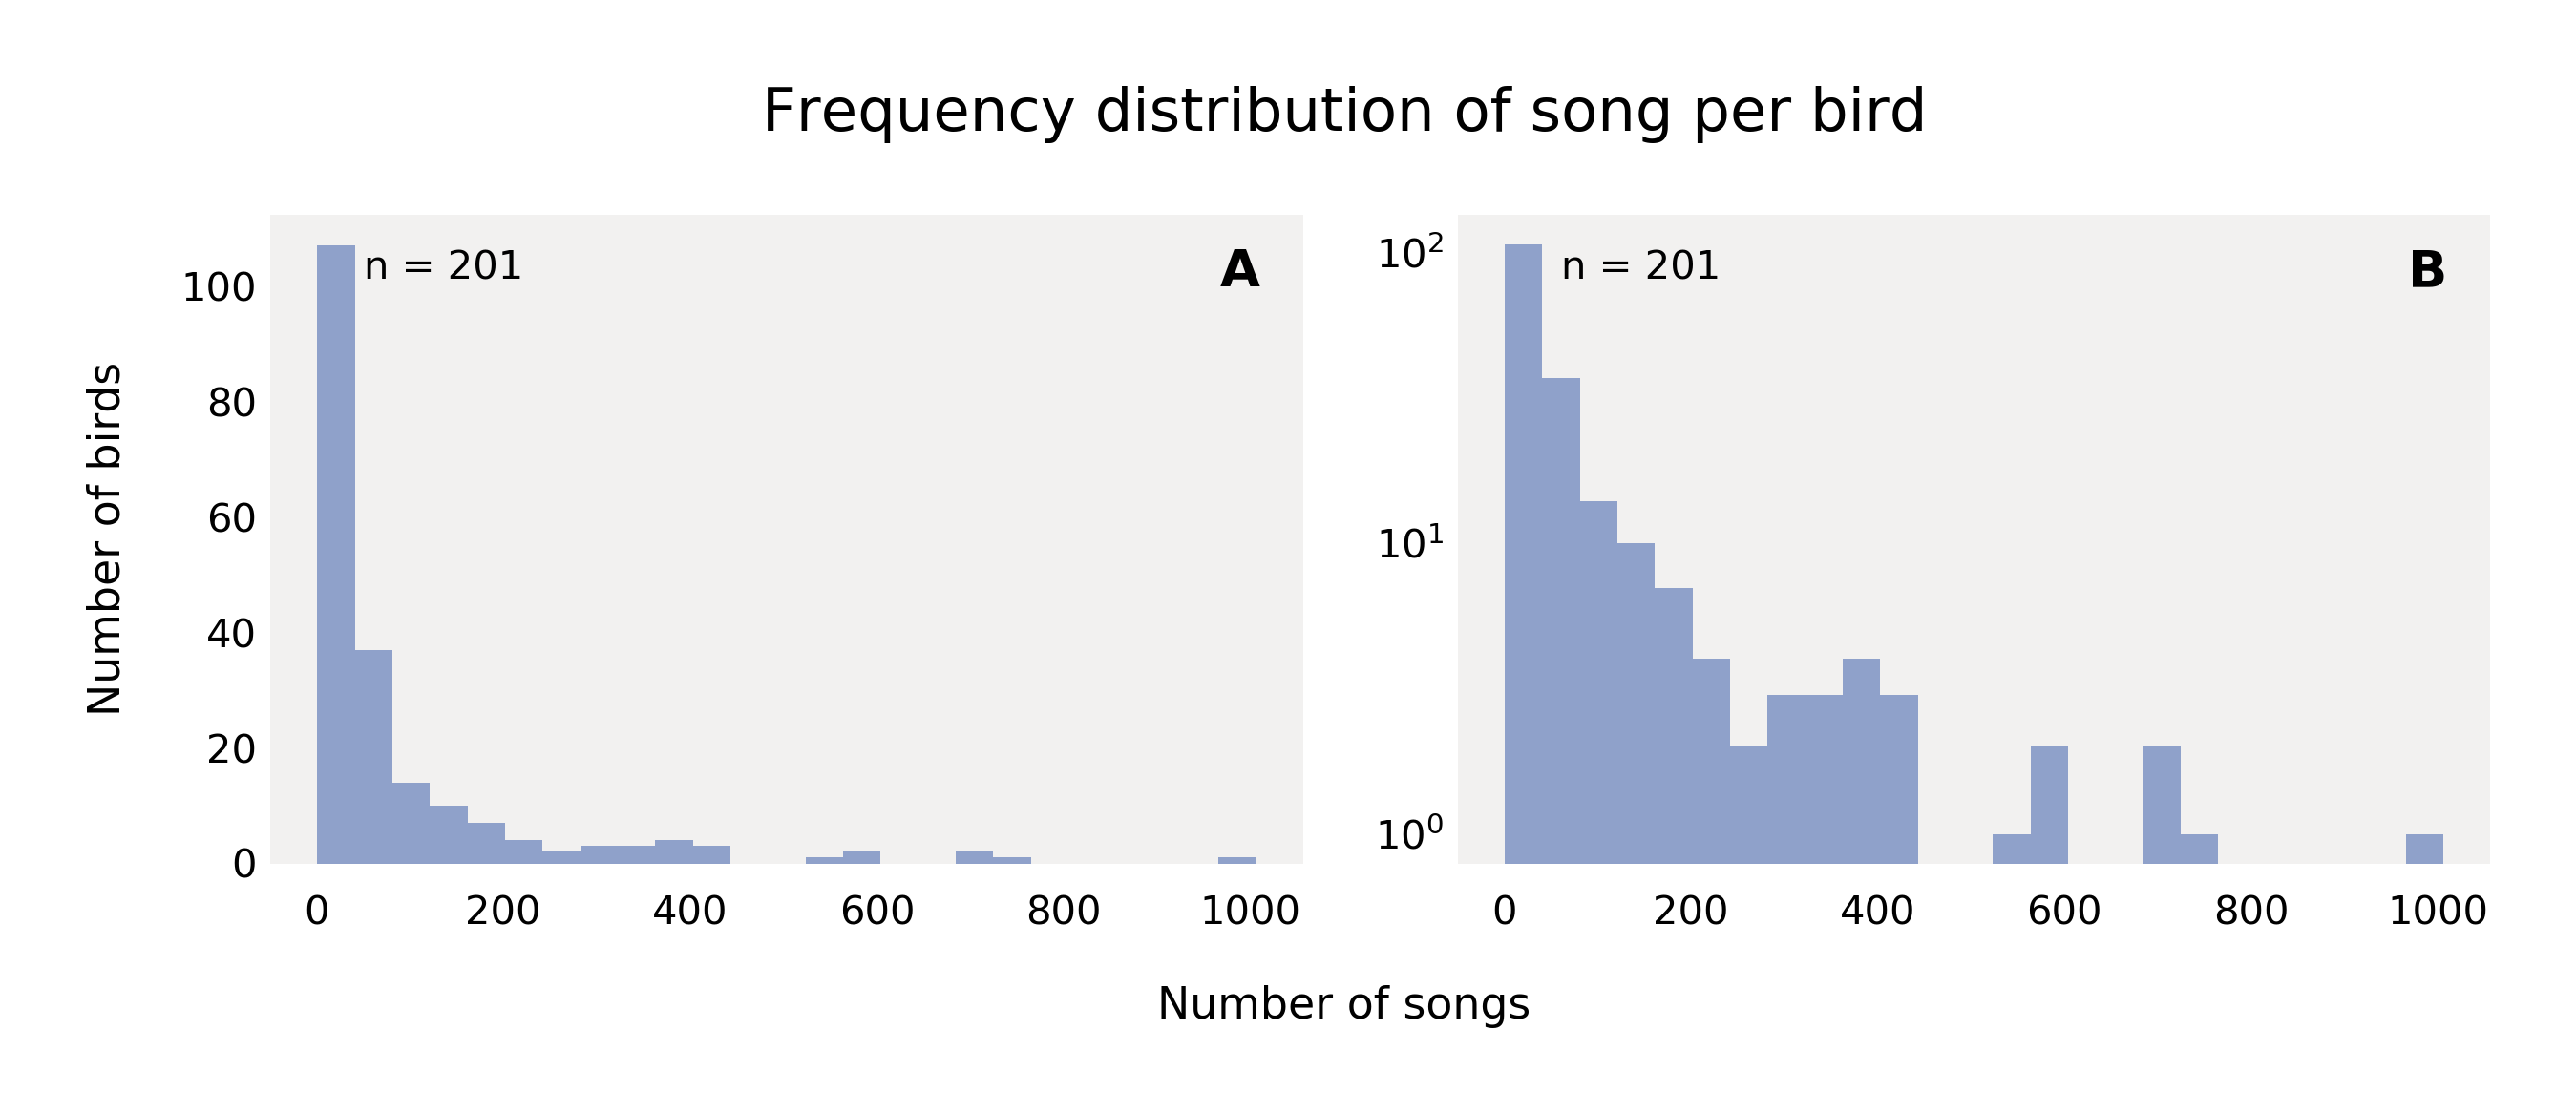
\includegraphics{../figures/2020/population/Frequency_distribution_song_n_2020-09-25_14:59.png}
\caption{Frequency distribution of the number of songs recorded per
bird}
\end{figure}

\begin{figure}
\centering
\includegraphics{../figures/population/phate.png}
\caption{PHATE projection of every note in the dataset}
\end{figure}

\hypertarget{songs-and-notes}{%
\subsection{Songs and notes}\label{songs-and-notes}}

Duration and frequency range statistics for the notes in the dataset,
quantifying individual variation.

Distribution of number of note types in the population

\begin{figure}
\centering
\includegraphics{../figures/2020/ind_repertoires/B3_repertoire_2020-09-22_17:36:53.png}
\caption{Example of the repertoire of a single bird}
\end{figure}

\begin{figure}
\centering
\includegraphics{../figures/2020/population/syllable_duration_pd_2020-10-04_14:39.png}
\caption{KDE of the distribution of note duration for every bird}
\end{figure}

\begin{figure}
\centering
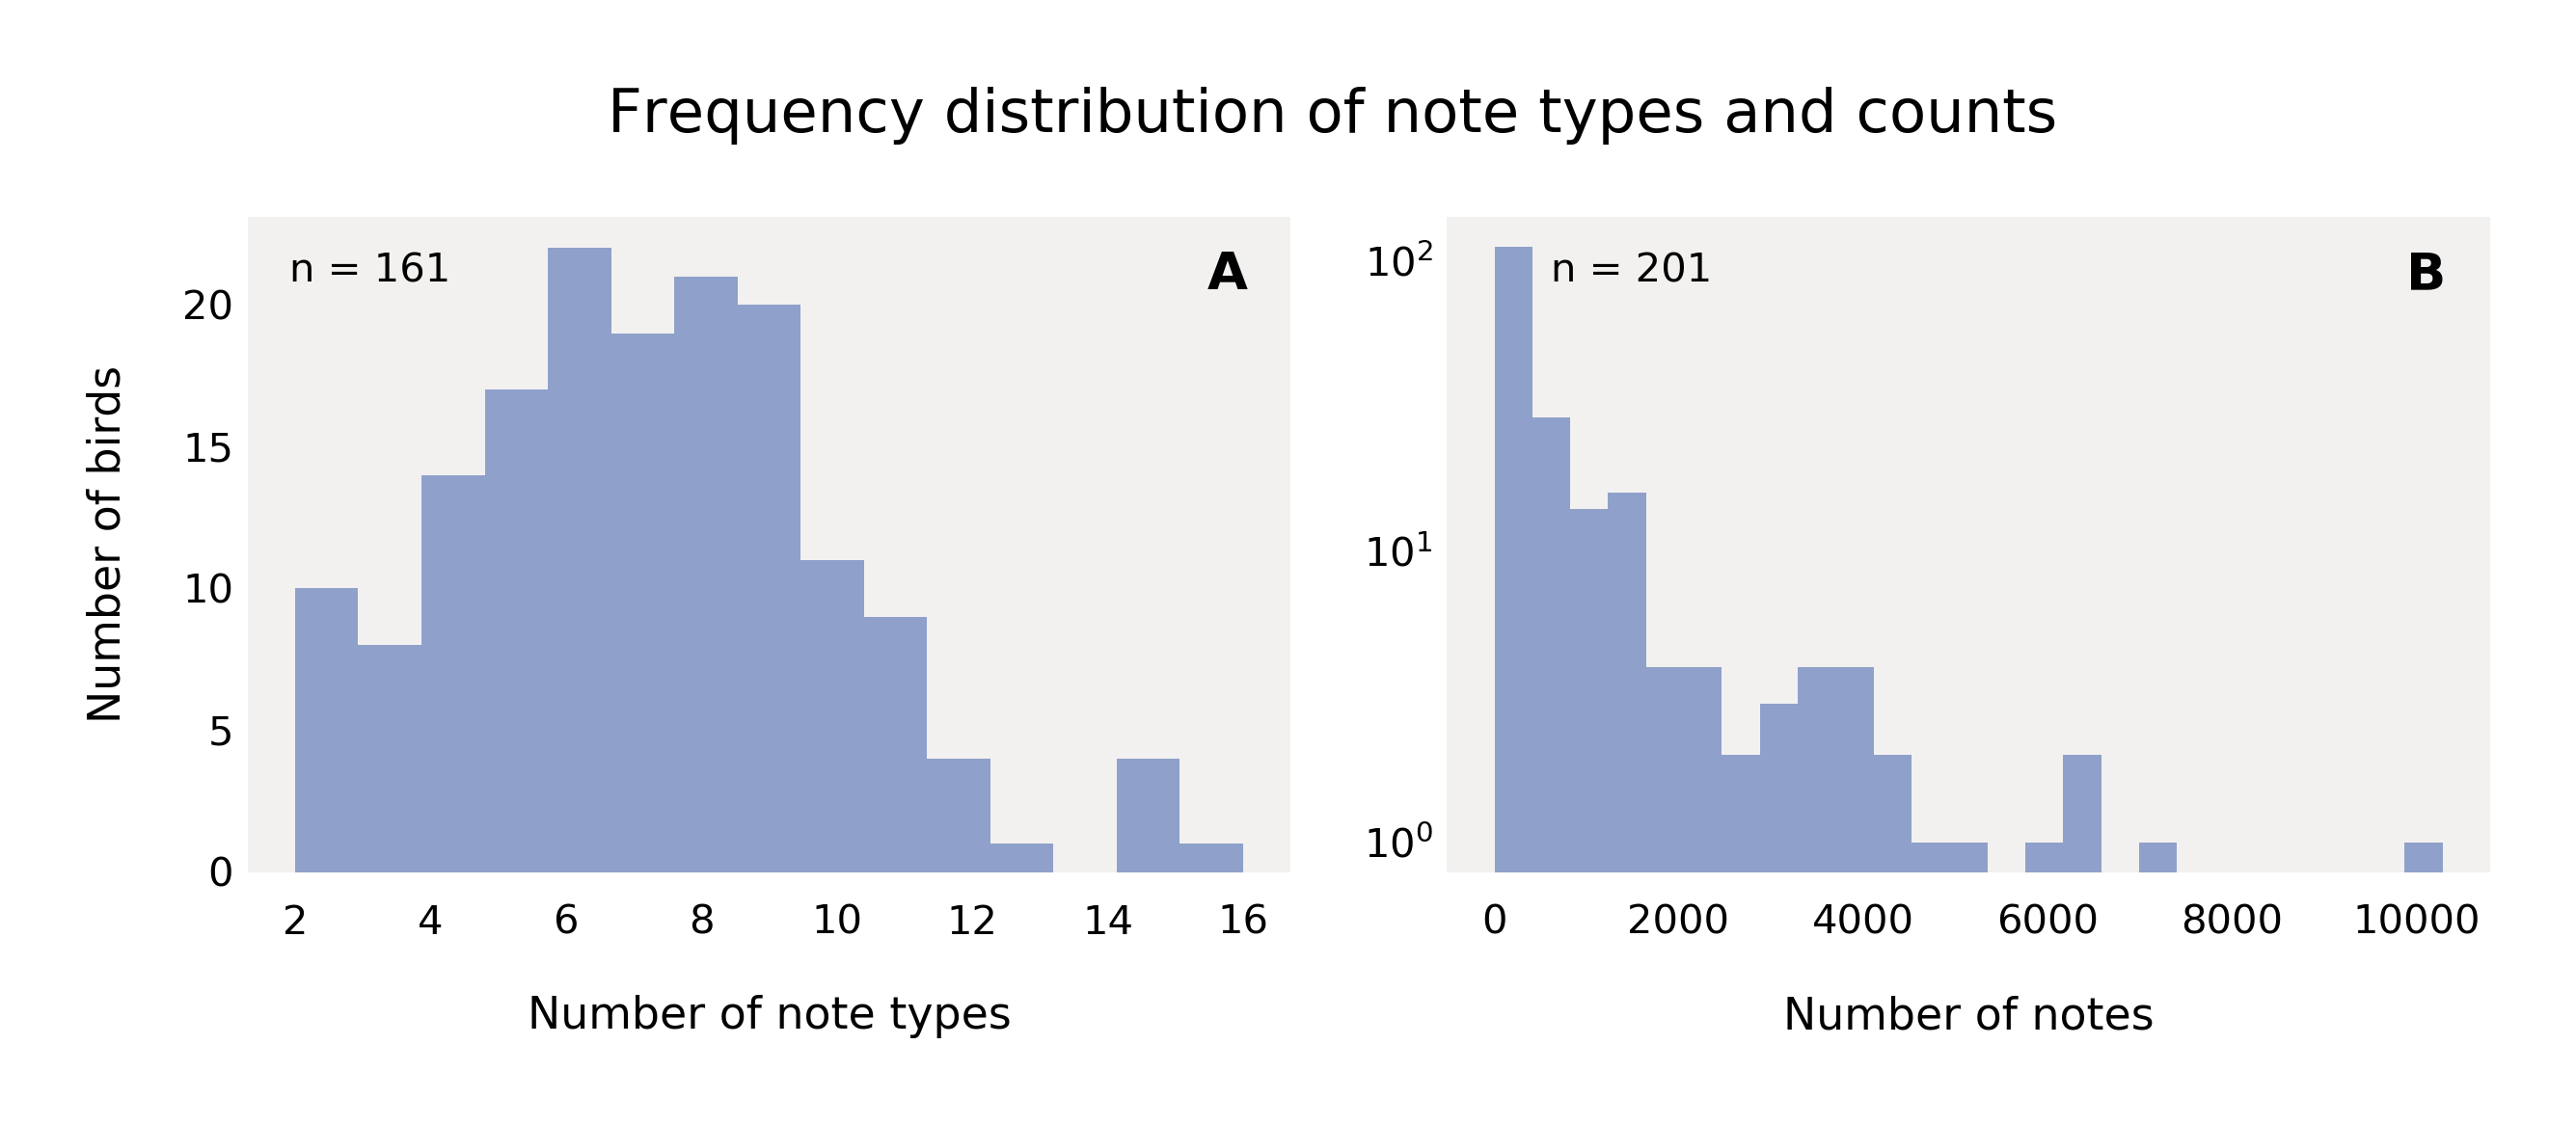
\includegraphics{../figures/2020/population/Frequency_distribution_note_types_2020-09-28_11:36.png}
\caption{Frequency distribution of note types and counts in the
population}
\end{figure}

\hypertarget{modelling-sampling-success}{%
\subsection{Modelling sampling
success}\label{modelling-sampling-success}}

Parameter estimates for models with number of songs recorded as outcome;
briefly,

\begin{itemize}
\item
  More lag from lay date = fewer songs,
\item
  Later lay date = fewer songs,
\item
  Father subsequently not ID'd = more likely to have 0 songs,
\end{itemize}

Cumulative curves for each male (number of songs recorded vs number of
note types)

\begin{figure}
\centering
\includegraphics{../figures/2020/population/pp_plot_n_songs.png}
\caption{Comparison of \(y\) to simulated datasets \(y^{rep}\) from the
posterior predictive distribution}
\end{figure}

\begin{figure}
\centering
\includegraphics{../figures/2020/population/post_plot.png}
\caption{Posterior distribution of model parameters}
\end{figure}

\hypertarget{data-collection-plan-for-2021}{%
\chapter{Data collection plan for
2021}\label{data-collection-plan-for-2021}}

What can be done to make sampling more successful in light of the
results above? This will be a brief discussion, the main points as
follows:

\begin{itemize}
\item
  There is a sharp decrease in singing activity towards the end of egg
  laying - much sharper than it seemed to me from the literature, but
  actually matches results from Mace
  (\protect\hyperlink{ref-Mace1987}{1987}).
\item
  Birds in nests with later lay dates also sing less, but the main
  correlate of sampling success is time passed since the onset of egg
  laying. In 2020 I was not able to place more than 10 recorders per
  day, but for a brief period (\textasciitilde{}4 days) I would have
  needed to place \textasciitilde{}35 every day. I didn't recover from
  the accumulated lag until almost the end of the recording period.
\item
  Therefore, an effort should be made to reduce this lag.
\item
  This requires:

  \begin{enumerate}
  \def\labelenumi{\alph{enumi})}
  \item
    earlier detection of nests with great tit activity, and
  \item
    better ability to cope with the influx of nests.
  \end{enumerate}
\item
  I will discuss potential solutions for a and b.
\end{itemize}

~ ~

\textbf{Outstanding Issues}

Winter social network data?

\hypertarget{thesis-plan}{%
\chapter{Thesis plan}\label{thesis-plan}}

\hypertarget{introduction-1}{%
\section{Introduction}\label{introduction-1}}

The introduction will provide a general background to the topic of song
learning in birds. I will try to integrate ideas from three bodies of
research that are sometimes disconnected: laboratory studies of song
ontogeny, behavioural ecology and cultural evolutionary theory. The
structure will be an iteration of the
\protect\hyperlink{introduction}{introduction} above.

\hypertarget{what-do-great-tits-sing}{%
\section{1. What do great tits sing?}\label{what-do-great-tits-sing}}

An in-depth description of the variability and similarity of great tit
songs, from an acoustic and information-theoretic perspective. This will
include a very detailed case study from the Wytham population and
comparison with data from across the distribution range of the species.

Questions include:

\begin{itemize}
\tightlist
\item
  Are `song types' meaningful categories at larger spatial scales?
\item
  Which song traits, from the level of notes to sequential organisation,
  are more constrained, and which more free to vary? Is variation
  stochastic?
\end{itemize}

\hypertarget{song-learning-and-learning-biases}{%
\section{2. Song learning and learning
biases}\label{song-learning-and-learning-biases}}

An exploration of the landscape of learning in the study population.

Questions include:

\begin{itemize}
\item
  Can the pattern of song sharing be explained in terms of unbiased
  learning plus the effects of population structure, immigration and
  dispersal, or does it require further assumptions?
\item
  Are all songs equally likely to be learnt? Is there evidence for
  frequency dependence in great tit song learning?
\item
  Are all males equally likely to serve as tutors?
\item
  There is no evidence that repertoire composition or size are
  inheritable in great tits. Work done in the lab with other species
  suggests that birds might be better at learning songs that are similar
  in tempo to those of their fathers. Is there any evidence for this in
  a wild population?
\item
  Is there a trade-off between repertoire size and repertoire
  complexity?
\end{itemize}

\hypertarget{space-and-demography}{%
\section{3. Space and demography}\label{space-and-demography}}

\begin{itemize}
\tightlist
\item
  How well does community structure predict acoustic structure at
  different scales?
\item
  Do any song characteristics change with population density?
\item
  How is the rate of acoustic change affected by population turnover
  rates?
\item
  Does being neighbours with more immigrant birds lead to (a) increased
  acoustic diversity or (b) having larger repertories?
\end{itemize}

\hypertarget{copying-fidelity-and-convergence-in-bird-song}{%
\section{4. Copying fidelity and convergence in bird
song}\label{copying-fidelity-and-convergence-in-bird-song}}

Many studies of bird song have concluded that learning is often
extremely accurate, with some even estimating that syllable types can
persist for longer than 500 years (e.g., Lachlan et al.
\protect\hyperlink{ref-Lachlan2018b}{2018}). Although accurate learning
does occur, as laboratory studies show, the fact that innate biases
alone can give rise to many species-typical song characteristics, even
in isolate, deafened, and self-tutored birds (Fehér et al.
\protect\hyperlink{ref-Feher2009}{2009},
\protect\hyperlink{ref-Feher2017}{2017}; James2017d; James et al.
\protect\hyperlink{ref-James2020}{2020}), suggests that strong
convergent transformation during song ontogeny might difficult the
estimation of mutation rates. I will explore this by fitting
individual-based simulation models of song change to empirical data
gathered in the Wytham population over three years.

\hypertarget{the-function-of-songs}{%
\section{5. The function of songs}\label{the-function-of-songs}}

Having a large dataset of songs matched to known individuals will allow
us to test questions relating to the current fitness consequences of
song-sharing and song performance.

\begin{itemize}
\tightlist
\item
  Is song-sharing beneficial? For whom? Is singing 'popular' songs
  beneficial for males?
\item
  Is spectrotemporal consistency in song performance positively
  correlated with reproductive success? What about small deviation from
  small integer ratios in the relationship between note frequencies?
\item
  If there is a relationship between repertoire size or degree of
  song-sharing with neighbours and RS, is this mediated by territory
  quality?
\item
  Does song production senesce? Are any song traits reliable signals of
  age?
\end{itemize}

\hypertarget{synthesis}{%
\section{Synthesis}\label{synthesis}}

A summary integrating the results of every chapter and situating them in
a broader theoretic context.

\hypertarget{references}{%
\chapter*{References}\label{references}}
\addcontentsline{toc}{chapter}{References}

\hypertarget{refs}{}
\leavevmode\hypertarget{ref-Allen2013a}{}%
\textbf{Allen, J., Weinrich, M., Hoppitt, W. \& Rendell, L.} 2013.
Network-based diffusion analysis reveals cultural transmission of
lobtail feeding in humpback whales. \emph{Science}, \textbf{340},
485--488.

\leavevmode\hypertarget{ref-Aplin2018}{}%
\textbf{Aplin, L. M.} 2019. Culture and cultural evolution in birds: a
review of the evidence. \emph{Animal Behaviour}, \textbf{147}, 179--187.

\leavevmode\hypertarget{ref-Burkner2017a}{}%
\textbf{Bürkner, P.-C.} 2017. brms : An R Package for Bayesian
Multilevel Models Using Stan. \emph{Journal of Statistical Software},
\textbf{80},

\leavevmode\hypertarget{ref-Carvalho2008}{}%
\textbf{Carvalho, S., Cunha, E., Sousa, C. \& Matsuzawa, T.} 2008.
Chaînes opératoires and resource-exploitation strategies in chimpanzee
(Pan troglodytes) nut cracking. \emph{Journal of Human Evolution},
\textbf{55}, 148--163.

\leavevmode\hypertarget{ref-Falotico2019}{}%
\textbf{Falótico, T., Proffitt, T., Ottoni, E. B., Staff, R. A. \&
Haslam, M.} 2019. Three thousand years of wild capuchin stone tool use.
\emph{Nature Ecology and Evolution},

\leavevmode\hypertarget{ref-Fayet2014}{}%
\textbf{Fayet, A. L., Tobias, J. A., Hintzen, R. E. \& Seddon, N.} 2014.
Immigration and dispersal are key determinants of cultural diversity in
a songbird population. \emph{Behavioral Ecology}, \textbf{25}, 744--753.

\leavevmode\hypertarget{ref-Feher2009}{}%
\textbf{Fehér, O., Wang, H., Saar, S., Mitra, P. P. \& Tchernichovski,
O.} 2009. De novo establishment of wild-type song culture in the zebra
finch. \emph{Nature}, \textbf{459}, 564--568.

\leavevmode\hypertarget{ref-Feher2017}{}%
\textbf{Fehér, O., Ljubičić, I., Suzuki, K., Okanoya, K. \&
Tchernichovski, O.} 2017. Statistical learning in songbirds: from
self-tutoring to song culture. \emph{Philosophical Transactions of the
Royal Society B: Biological Sciences}, \textbf{372}, 20160053.

\leavevmode\hypertarget{ref-Galef2005}{}%
\textbf{Galef, B. G. \& Laland, K. N.} 2005 June. Social learning in
animals: Empirical studies and theoretical models. \textbf{55},
489--499.

\leavevmode\hypertarget{ref-Giraldeau2002}{}%
\textbf{Giraldeau, L. A., Valone, T. J. \& Templeton, J. J.} 2002
November. Potential disadvantages of using socially acquired
information. \textbf{357}, 1559--1566.

\leavevmode\hypertarget{ref-Henrich1998}{}%
\textbf{Henrich, J. \& Boyd, R.} 1998. The Evolution of Conformist
Transmission and the Emergence of Between-Group Differences.
\emph{Evolution and Human Behavior}, \textbf{19}, 215--241.

\leavevmode\hypertarget{ref-Hill2019b}{}%
\textbf{Hill, A. P., Prince, P., Snaddon, J. L., Doncaster, C. P. \&
Rogers, A.} 2019. AudioMoth: A low-cost acoustic device for monitoring
biodiversity and the environment. \emph{HardwareX}, \textbf{6}, e00073.

\leavevmode\hypertarget{ref-Hinde1952}{}%
\textbf{Hinde, R. A.} 1952. The Behaviour of the Great Tit (Parus major)
and Some Other Related Species. \emph{Behaviour. Supplement},
\textbf{2}, III--201.

\leavevmode\hypertarget{ref-Hunter1979}{}%
\textbf{Hunter, M. L. \& Krebs, J. R.} 1979. Geographical Variation in
the Song of the Great Tit (Parus major) in Relation to Ecological
Factors. \emph{Journal of Animal Ecology}, \textbf{48}, 759--785.

\leavevmode\hypertarget{ref-James2020}{}%
\textbf{James, L. S., Davies, R., Mori, C., Wada, K. \& Sakata, J. T.}
2020. Manipulations of sensory experiences during development reveal
mechanisms underlying vocal learning biases in zebra finches.
\emph{Developmental Neurobiology}, \textbf{80}, 132--146.

\leavevmode\hypertarget{ref-Krebs1978}{}%
\textbf{Krebs, J., Ashcroft, R. \& Webber, M.} 1978. Song repertoires
and territory defence in the great tit. \emph{Nature}, \textbf{271},
539--542.

\leavevmode\hypertarget{ref-Lachlan2018b}{}%
\textbf{Lachlan, R. F., Ratmann, O. \& Nowicki, S.} 2018. Cultural
conformity generates extremely stable traditions in bird song.
\emph{Nature Communications}, \textbf{9}, 2417.

\leavevmode\hypertarget{ref-Laland2003}{}%
\textbf{Laland, K. N. \& Hoppitt, W.} 2003. Do Animals Have Culture?
\emph{Evolutionary Anthropology}, \textbf{12}, 150--159.

\leavevmode\hypertarget{ref-Mace1987}{}%
\textbf{Mace, R.} 1987. The dawn chorus in the great tit Parus major is
directly related to female fertility. \emph{Nature}, \textbf{330},
745--746.

\leavevmode\hypertarget{ref-Marsland2019}{}%
\textbf{Marsland, S., Priyadarshani, N., Juodakis, J. \& Castro, I.}
2019. AviaNZ: A future-proofed program for annotation and recognition of
animal sounds in long-time field recordings. \emph{Methods in Ecology
and Evolution}, \textbf{10}, 1189--1195.

\leavevmode\hypertarget{ref-McGregor1982}{}%
\textbf{McGregor, P. K. \& Krebs, J. R.} 1982. Song Types in a
Population of Great Tits (Parus major): Their Distribution, Abundance
and Acquisition by Individuals. \emph{Behaviour}, \textbf{79}, 126--152.

\leavevmode\hypertarget{ref-McGregor1989}{}%
\textbf{McGregor, P. K. \& Krebs, J. R.} 1989. Song learning in adult
great tits (Parus major): effects of neighbours. \emph{Behaviour},
\textbf{108}, 139--159.

\leavevmode\hypertarget{ref-McInnes2017}{}%
\textbf{McInnes, L., Healy, J. \& Astels, S.} 2017. hdbscan:
Hierarchical density based clustering. \emph{The Journal of Open Source
Software}, \textbf{2}, 205.

\leavevmode\hypertarget{ref-McInnes2018}{}%
\textbf{McInnes, L., Healy, J. \& Melville, J.} 2018. UMAP: Uniform
Manifold Approximation and Projection for Dimension Reduction. \emph{The
Journal of Open Source Software}, \textbf{3}, 861.

\leavevmode\hypertarget{ref-Mercader2007}{}%
\textbf{Mercader, J., Barton, H., Gillespie, J., Harris, J., Kuhn, S.,
Tyler, R. \& Boesch, C.} 2007. 4,300-Year-old chimpanzee sites and the
origins of percussive stone technology. \emph{Proceedings of the
National Academy of Sciences of the United States of America},
\textbf{104}, 3043--3048.

\leavevmode\hypertarget{ref-Mets2017}{}%
\textbf{Mets, D. G. \& Brainard, M. S.} 2017. Genetic variation
interacts with experience to determine interindividual differences in
learned song. \emph{Proceedings of the National Academy of Sciences of
the United States of America}, \textbf{115}, 421--426.

\leavevmode\hypertarget{ref-Mets2018}{}%
\textbf{Mets, D. G. \& Brainard, M. S.} 2018. An automated approach to
the quantitation of vocalizations and vocal learning in the songbird.
\emph{PLoS Computational Biology}, \textbf{14}, e1006437.

\leavevmode\hypertarget{ref-Mets2019}{}%
\textbf{Mets, D. G. \& Brainard, M. S.} 2019. Learning is enhanced by
tailoring instruction to individual genetic differences. \emph{eLife},
\textbf{8}, 1--15.

\leavevmode\hypertarget{ref-Moon2019}{}%
\textbf{Moon, K. R., Dijk, D. van, Wang, Z., Gigante, S., Burkhardt, D.
B., Chen, W. S., Yim, K., Elzen, A. van den, Hirn, M. J., Coifman, R.
R., Ivanova, N. B., Wolf, G. \& Krishnaswamy, S.} 2019. Visualizing
structure and transitions in high-dimensional biological data.
\emph{Nature Biotechnology}, \textbf{37}, 1482--1492.

\leavevmode\hypertarget{ref-Perrins1965}{}%
\textbf{Perrins, C. M.} 1965. Population Fluctuations and Clutch-Size in
the Great Tit, Parus major L. \emph{Journal of Animal Ecology},
\textbf{34}, 601--647.

\leavevmode\hypertarget{ref-Perry2003}{}%
\textbf{Perry, S., Baker, M., Fedigan, L., Gros-Louis, J., Jack, K.,
MacKinnon, K. C., Manson, J. H., Panger, M., Pyle, K. \& Rose, L.} 2003.
Social conventions in wild white-faced capuchin monkeys: Evidence for
traditions in a neotropical primate. \emph{Current Anthropology},
\textbf{44}, 241--268.

\leavevmode\hypertarget{ref-Sainburg2019b}{}%
\textbf{Sainburg, T., Theilman, B., Thielk, M. \& Gentner, T. Q.} 2019.
Parallels in the sequential organization of birdsong and human speech.
\emph{Nature Communications}, \textbf{10},

\leavevmode\hypertarget{ref-Sasaki2017a}{}%
\textbf{Sasaki, T. \& Biro, D.} 2017. Cumulative culture can emerge from
collective intelligence in animal groups. \emph{Nature Communications},
\textbf{8}, 15049.

\leavevmode\hypertarget{ref-Searfoss2020}{}%
\textbf{Searfoss, A. M., Pino, J. C. \& Creanza, N.} 2020. Chipper:
Open-source software for semi-automated segmentation and analysis of
birdsong and other natural sounds. \emph{Methods in Ecology and
Evolution}, \textbf{11}, 524--531.

\leavevmode\hypertarget{ref-Slater2003}{}%
\textbf{Slater, P. J.} 2003. Fifty years of bird song research: A case
study in animal behaviour. \emph{Animal Behaviour}, \textbf{65},
633--639.

\leavevmode\hypertarget{ref-Tchernichovski2017a}{}%
\textbf{Tchernichovski, O., Feher, O., Fimiarz, D. \& Conley, D.} 2017.
How social learning adds up to a culture: from birdsong to human public
opinion. \emph{The Journal of Experimental Biology}, \textbf{220},
124--132.

\leavevmode\hypertarget{ref-Whitehead2009}{}%
\textbf{Whitehead, H. \& Richerson, P. J.} 2009. The evolution of
conformist social learning can cause population collapse in
realistically variable environments. \emph{Evolution and Human
Behavior}, \textbf{30}, 261--273.

\leavevmode\hypertarget{ref-Whiten2017}{}%
\textbf{Whiten, A., Ayala, F. J., Feldman, M. W. \& Laland, K. N.} 2017.
The extension of biology through culture. \emph{Proceedings of the
National Academy of Sciences of the United States of America},
\textbf{114}, 7775--7781.

\end{document}
